Projektina on tarkoitus toteuttaa sovellus Mafioso-seura/roolipelistä. Sovellus
on ensisijaisesti tukevana apuna pelissä, mutta voi mahdollistaa pelin
vetämisen täyden automaatioinnin ajan myötä.

\section{Mafioso-pelin idea/säännöt}

Mafiosossa jokaiselle osallistujalle jaetaan joku rooli. Rooli määrittää
pelaajan toimia ja tavoitteita pelissä. Peliä etenee yö-päivä -sykleissä,
joissa öisin tapahtuu muiden tietämättä asioita ja päivisin yritetään ratkaista
puhumalla ja kyselemällä mitä on tapahtunut ja ketkä ovat syyllisiä. Pelissä on
tarkoitus saada pelaajista koostuvasta kyläyhteisestä äänestettyä päivien
aikana pois ns. pahat henkilöt, ennen kuin kyseiset henkilöt ehtivät öisin
pudottaa ns. hyvät henkilöt.

Yleisimpiä rooleja ovat kansalainen, mafia, poliisi, lääkäri ja hullu. Rooleja
riittää toki vaikka kuinka paljon, mutta esitellään tässä vain muutamat
yleiseimmistä, jotta asiat saadaan pidettyä yksinkertaisina.

Kansalaisen rooli on hyvinkin yksinkertainen. Kansalainen nukkuu koko yön eikä
tee öisin mitään. Päivisin kansalainen yrittää yhdessä muun kyläyhteisön kanssa
saada selville ketkä ovat pahojen puolella ja äänestää heidät pois pelistä.

Mafiat herätään yöllä muiden nukkuessa. Mafia pääsevät kaikki olemaan hereillä
yhtä aikaa ja näkevät toisensa. Mafiat päättävät yöllä yhdessä kuka pelaajista
heitetään pois pelistä. Päivisin Mafiat yrittävät huijata ja juonitella
kansalaiset äänestämään muita kansalaisia pois ja pyrkivät estämään, ettei
mafiaa äänestetä pois.

Poliisi herää yöllä yksin ja pääsee "skannaamaan" yhden henkilön. Poliisi saa
tietää kyseisestä henkilöstä onko hän hyvä (kaikki ei pahat) vai paha (joihin
kuuluu mafia ja poliisi (toki poliisi on oikeasti hyvä, mutta skannaus näyttää
pahana)). Päivisin poliisi voi kertoa saamiaan tuloksia ja saada kansan
mahdollisesti äänestämään pahoja pois, mutta asettaa samalla itsensä vaaraan
paljastaessaan olevansa poliisi.

Lääkäri herää myös yöllä yksin ja pääsee pelastamaan yhden henkilön. Valittu
henkilö ei voi pudota yöllä mafian tai hullun toimesta. Yleensä varsinkin
alkupelissä lääkäri pelastaa itsensä, mutta jatkossa esim. paljastuneen
poliisin suojeleminen voi olla myös vaihtoehto. Päivisin lääkäri on kuten
tavallinen kansalainen.

Hullu hereilee yöllä yksin ja pääsee yksinään valitsemaan kenet heittää pihalle
pelistä. Päivisin hullu yrittää vain saada muita äänestämään muita pois ja
pidettyä itsensä pelissä.

Peli päättyy kun jäljellä on vain mafiaa, vain hullu yksin tai vain kansalaisia
tai muita hyviä roolea (lääkäri, poliisi). Voittajia ovat ne, ketkä ovat yhä
hengissä pelin päätyttyä.

Varsinainen pelaaminen tapahtuu yleensä kasvotusten istumalla piirissä.
Jokaiselle pelaajalle jaetaan pelikortti, jonka maa/arvo kuvastaa roolia.
Peliä johtaa yksi henkilö, joka itse ei ole mukana pelissä. Yön alettua
pelaajat sulkevat silmänsä, jonka jälkeen pelinjohtaja herättää yhden roolin
kerrallaan hereille. Rooli tekee toimintonsa mahdollisimman hiljaa ja
huomaamatta. Toiminnot pystytään kaikki tekemään osoittamalla itseään tai
muita henkilöitä niin, että pelinjohtaja pystyy näkemään valinnan. Kun kaikki
roolit on käyty läpi, pyytää pelinjohtaja kaikkia pelaajia heräämään ja kertoo
mikä tilanne aamulla on (ketkä ovat pudonneet). Pelinjohtaja ei kerro kuka on
pudottanut ja kenen vaan ideana on että kylän herättyä aamuun löytävät he
kuolleina pelinjohtajan mainitsemat pelaajat tietämättä asiasta sen enempää.
Päivisin pidetään puheenvuoroja ja äänestyksiä, kunnes lopulta enemistö haluaa
pudottaa yhden henkilön, jonka jälkeen pelaaja poistetaan pelistä ja siirrytään
yöhön. Vaihtoehtoisesti päivien kestäessä liian pitkään, voi pelinjohtaja
todeta auringon laskevan ja toivottaen kylälle hyvää yötä.

\subsection{Pelissä ilmevät käytännön ongelmat}

Peli toimii ideana melko hyvin kunhan roolit ovat saatu valittua sopivasti.
Kuitenkin käytännön toteutuksessa on välillä haasteita saada pidettyä peli
toimivana.

Isoilla pelaaja määrillä alussa roolien jakaminen ja määrittäminen
voi olla työlästä ja yhden lisäpelaajan ilmaantuminen voi viedä helposti 5-10
minuuttia ylimääräistä aikaa kun roolit pitää katsoa kokonaan uusiksi.
Vastaavasti yhden pelaajan lähteminen juuri kun roolit on jaettu, saattaa
muuttaa pelin tasapainoa sen verran, että roolit joudutaan valitsemaan
uudelleen.

Normaaleilla pelikorteilla pelattessa ei ole aina kaikille täysin selvää, minkä
roolin sai ja voi tämän seurauksena vahingossa paljastaa roolinsa ihmetellessä
mikä rooli tai mitä rooli tekee.

Isoilla määrillä on öiset toiminnot haastavia. Ei ole aina selvää ketä kukakin
osoittaa piirissä. Pelinjohtajalla on lisäksi hyvin paljon muistettavaa ja
huomioitavaa, kun isoilla määrillä otetaan yleensä huomattavasti enemmän
rooleja. Monet roolit sekoittavat öisiä tapahtumia merkittävästi ja kaikki
ei ole enää suoraviivaista.

Äänestystilanteiden olisi myös tarkoitus olla toisten äänetyksistä
riippumattomia, jotta mm. mafia ei voi vain lähteä mukaan kun näkee
muidenkin äänestävän, sillä äänestykset ovat julkisia, joten niiden avulla
voidaan perustella miksi joku voisi olla paha henkilö, jos aina äänestämässä
jotain pois. Myös tietyt roolit voivat tehdä äänenlaskennasta haastellisempaa
ylimääräisten äänien yms. vuoksi.

\subsection{Sovellukset tuomat ratkaisut ongelmiin}

Sovelluksen ideana on takertua mm. yllämainittuihin ongelmiin ja tuoda niihin
ratkaisua. Sovelluksen kehittyessä tavoitteena jopa mahdollistaa pelinjohtajan
kokonaan korvaaminen sovelluksella, jolloin yhtä henkilöä ei tarvitse sitoa
pelinjohtajan tehtävään vaan voi hänkin osallistua peliin. Pelinjohtajan rooli
vaatii myös paremman osaamisen pelistä, joten sovellus voi auttaa tilanteissa,
joissa pelinjohtaja ei ole kokenut henkilö.

\section{Projektin eteminen}

Projekti on toteutettu melko suoraviivaisesti suoraan käymällä tekemään
varsinaista sovellusta ilman sen tarkempaa suunnittelua. Lähtökohtaisesti
tavoitteena on saada alkuun toteutus, jolla on mahdollista pelata peli läpi,
mutta ainoastaan pienimmällä määrällä pakollisia toiminnallisuuksia. Voisi
osittain sanoa, että ideana on luoda prototyyppi, jota tosin lähdetään
kehittämään suoraan valmiiksi, jos vain jotenkin mahdollista.

\subsection{Projektin suunnittelu}

Projektin alkuperäinen hahmottelua on tapahtunut varmaankin vuonna 2019
keväällä. Tuolloin toki lähinnä ideana eikä niinkään miettien yksityiskohtia
sen enempää.

Alkuvuonna 2023 hiukan ennen kurssin alkua, alkoi asioiden ylöskirjaaminen
niistä kaikista toiminnallisuuksia ja huomioista, joita on tullut mieleen.
Tämäkin tosin ollut lähinnä 1-2 alkuyön mietiskelyjä hiukan ennen
nukkumista ja niiden ylöskirjaamista. Kyseiset muistiinpanot on nähtävissä
liittessä \ref{lst:mafioso-notes}.

\subsection{Projektin toteuttaminen}

Opiskelun sekä harjoitustehtävien tekemisen ja projektin koodaamisen
aloittamisen väliin jää useita viikkoja ja tässä välissä ehtii tulla uusi
versio niin Android Studiosta kuin Kotlinistakin.

Android Studion päivittämisen myötä templatet hiukan vaihtuvat
\parencite{AndroidStudioFlamingoReleaseNotes} ja aiheuttavan hämminkiä, mutta
muutaman yrityksen ja erehdyksen jälkeen saadaan luotua haluttu alustus
projektille. Muutoslokeja lukiessa huomasi päivityksen Live Edit
-toiminnallisuuteen, jonka myötä perehdyin siihen hiukan tarkemmin ja sain
käytettyä sitä projektia tehdessä. Jetback Composen esikatelut ovat toki
käteviä, mutta LiveEdit mahdollistaa todellisemmin muutosten näkemisen, kun ne
näkyvät suoraan emulaattorissa. Toki aina kaikkea ei ollut mahdollista
päivittää suoraan, mutta varsinkin komponenttien sijoittelut, välien
laittaminen ja muu vastaava tyylistys toimii hyvin LiveEditin kanssa.

Kotlin 1.9.0 versio julkaistiin oikeastaan jo aiemmin kun tein
harjoitustehtäviä, mutta tuolloin ei vielä vaikuttanut toimivan kunnolla
kääntäjälaajennus tms., mutta nyt sai asetettu kotlinCompilerExtensionVersion
-asetukseen version 1.5.0, joten saatiin käyttöön Kotlin 1.9.0.

Toteuttaminen on tarkoitus toteuttaa vaihe kerrallaan seuraavasti:
\begin{enumerate}
    \item Toteutetaan näkymät: etusivu, pelin luonti, peliin liittyminen ja
          varsinainen peli näkymä
    \item Lähetään sijoittelemaan näkymiin komponentteja
    \item Lisätään näkyviin toiminnallisuutta ViewModel avulla
    \item Lisätään pelin logiikkaa (mm. roolien arpomista, pelin loppumisen
          tarkistamista)
    \item Toteutetaan peliin liittyminen / kommunikointi usean puhelimen
          välillä
    \item Tallennetaan pelit (puhelimelle/pilveen)
    \item Toteutetaan aiemmien esiteltyihin käytännön haasteisiin ratkaisut
    \item Toteutetaan ylimääräisiä ominaisuuksia, joita muistiinpanoissa ja
          laajennetaan vanhoja
\end{enumerate}

Alkuun mallia saa katsottua hyvin CodeLabista
\parencite{AndroidDevelopersCodelabsComposeNavigation}. Tämän lisäksi aiemmin
tehdyistä muista Android kurssien tehtävistä sekä mobiliiohjelmointi kurssin
harjoitustehtävistä sai katsottua mallia. Lisäksi Jetback Composelle on tehty
useita toiminnallisuuksia kattavia esimerkkisovelluksia
\parencite{GithubAndroidComposeSamples}.

Valitettavasti jälleen aikataulun huono hallinta aiheutti hyvin rajallisen
määrän aikaa projektin tekemiseen. Projekti pääsi kurssin asettaman aikarajan
puitteissa toteuttamaan pelin logiikkaa sen verran, että sovelluksella on
mahdollista pelata peli läpi.

Kuvassa \ref{fig:screenshot-homescreen} on esillä aloitusnäkymä, josta pääsee
kahteen eri näkymään; uuden pelin luomiseen ja muiden luomien pelien
liittymiseen. Pelinluontinäkymässä (kuva \ref{fig:screenshot-create-game})
on mahdollista luoda uusi peli antamalla pelille nimi. Myöhemmin on tarkoitus
toteuttaa kuvassa \ref{fig:screenshot-join-game} näkyvään näkymään peliin
liittymislista, josta pääsee liittymään toisen luomaan peliin.

\begin{figure}[h!]
      \centering
      \begin{minipage}[t]{.3\textwidth}
            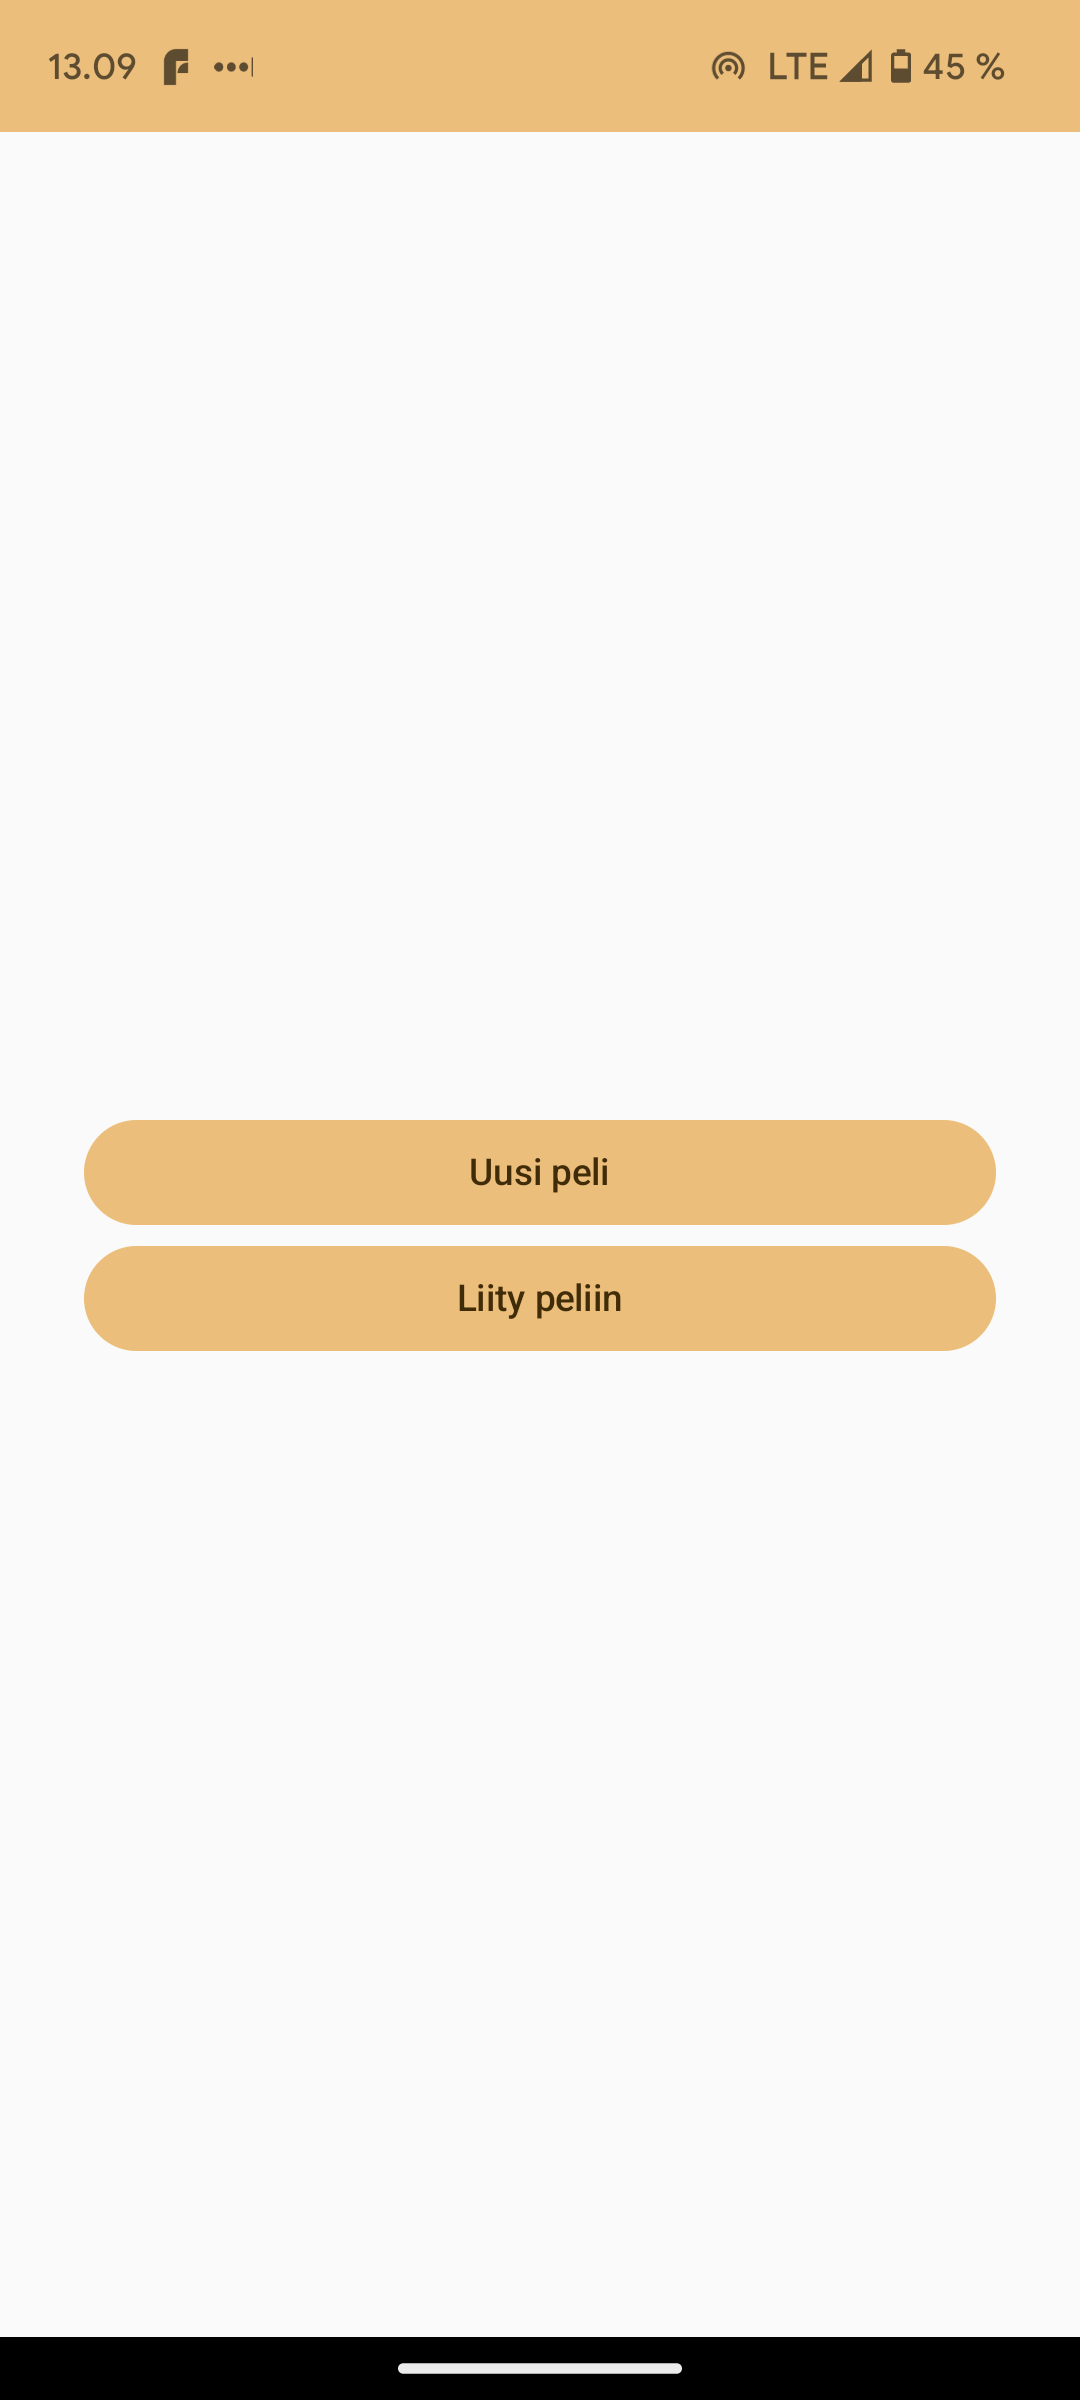
\includegraphics[width=\textwidth]{figures/screenshot-homescreen.png}
            \caption{Aloitusnäkymä}
            \label{fig:screenshot-homescreen}
      \end{minipage}
      \begin{minipage}[t]{.3\textwidth}
            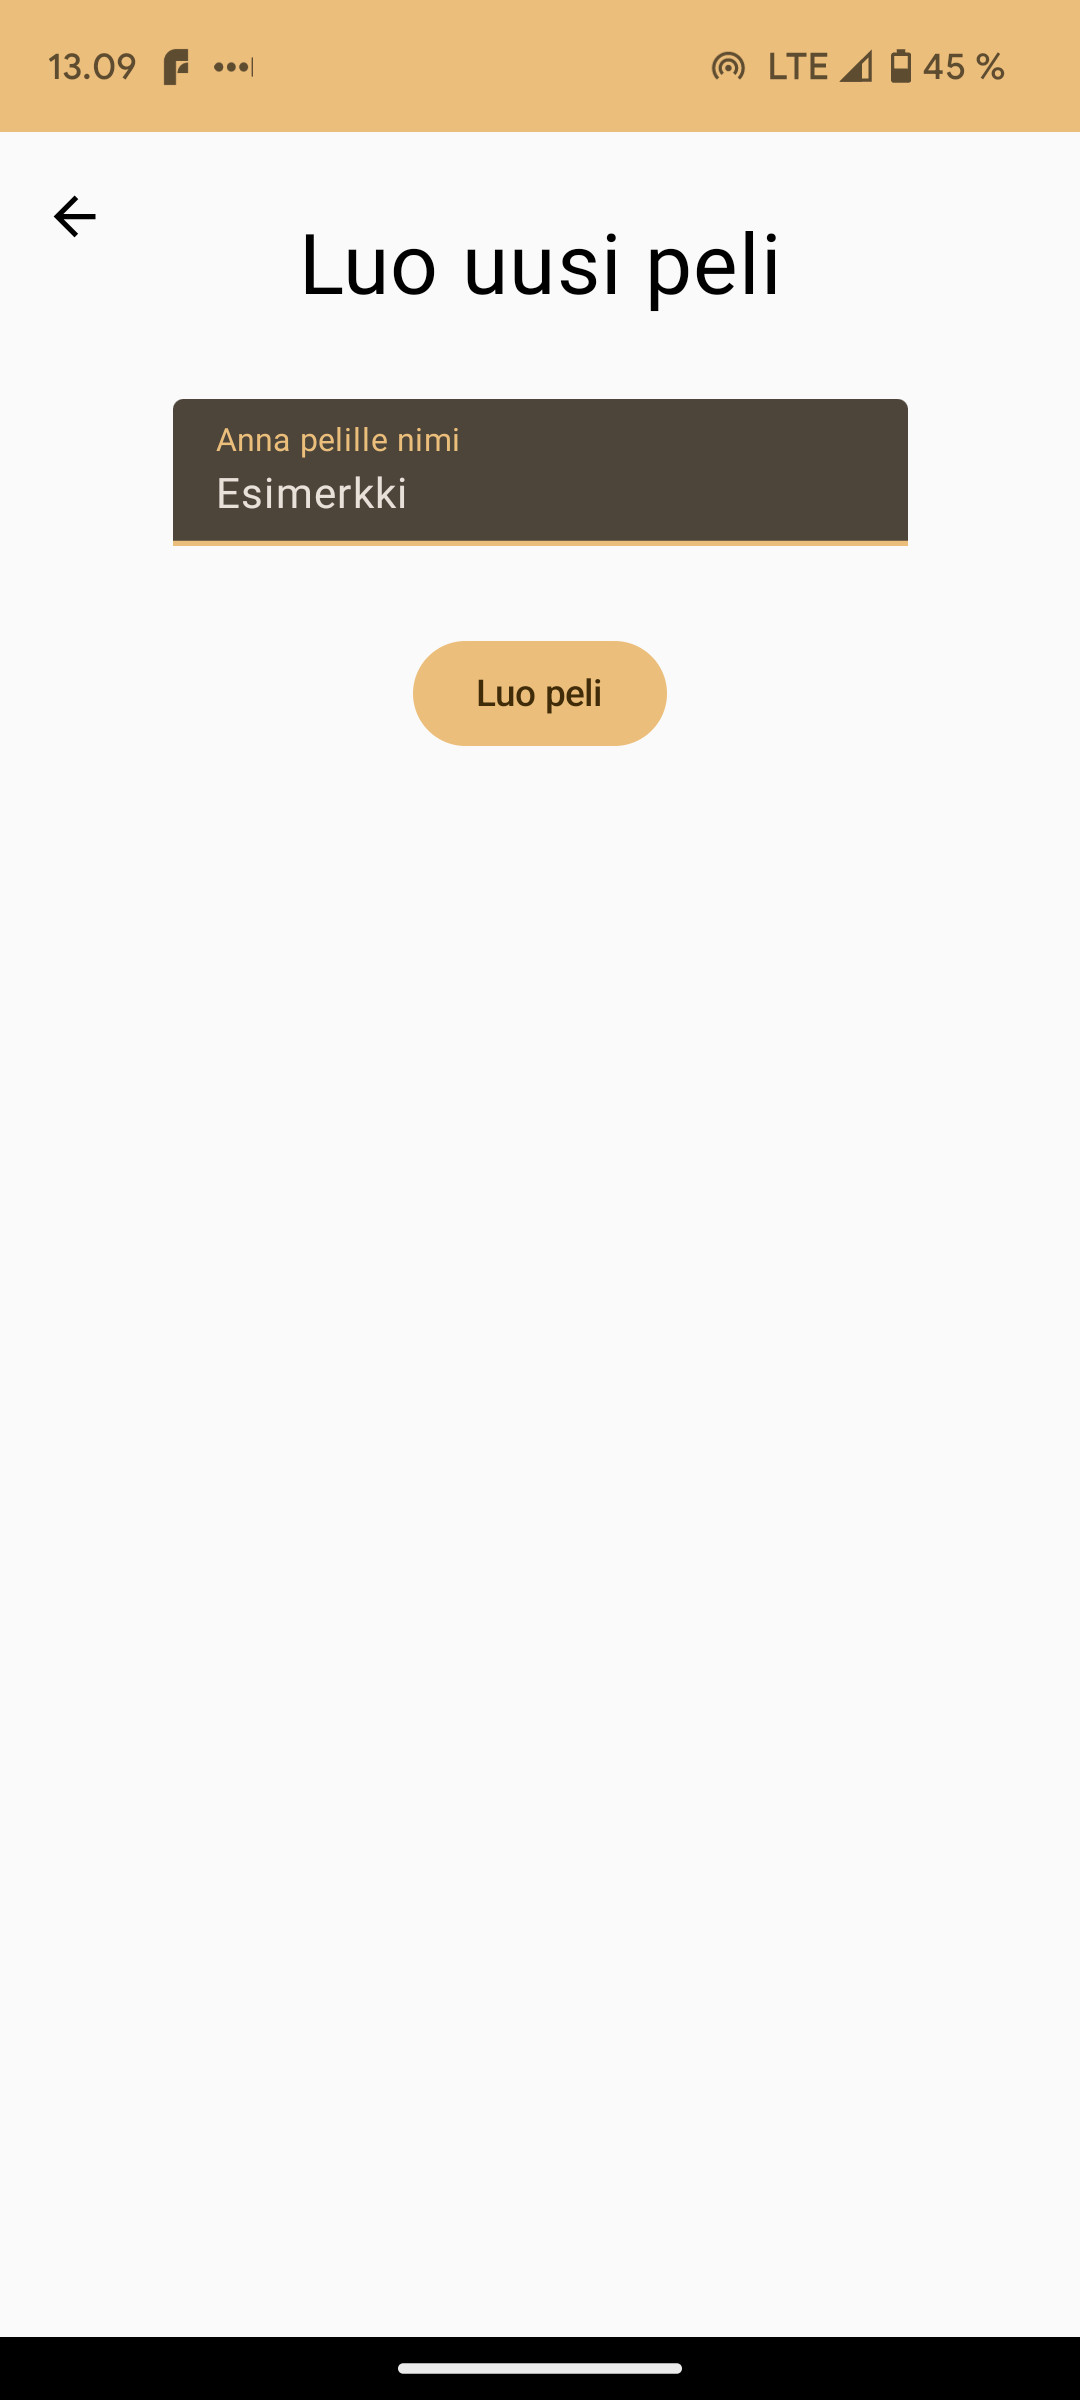
\includegraphics[width=\textwidth]{figures/screenshot-create-game.png}
            \caption{Pelinluontinäkymä}
            \label{fig:screenshot-create-game}
      \end{minipage}
      \begin{minipage}[t]{.3\textwidth}
            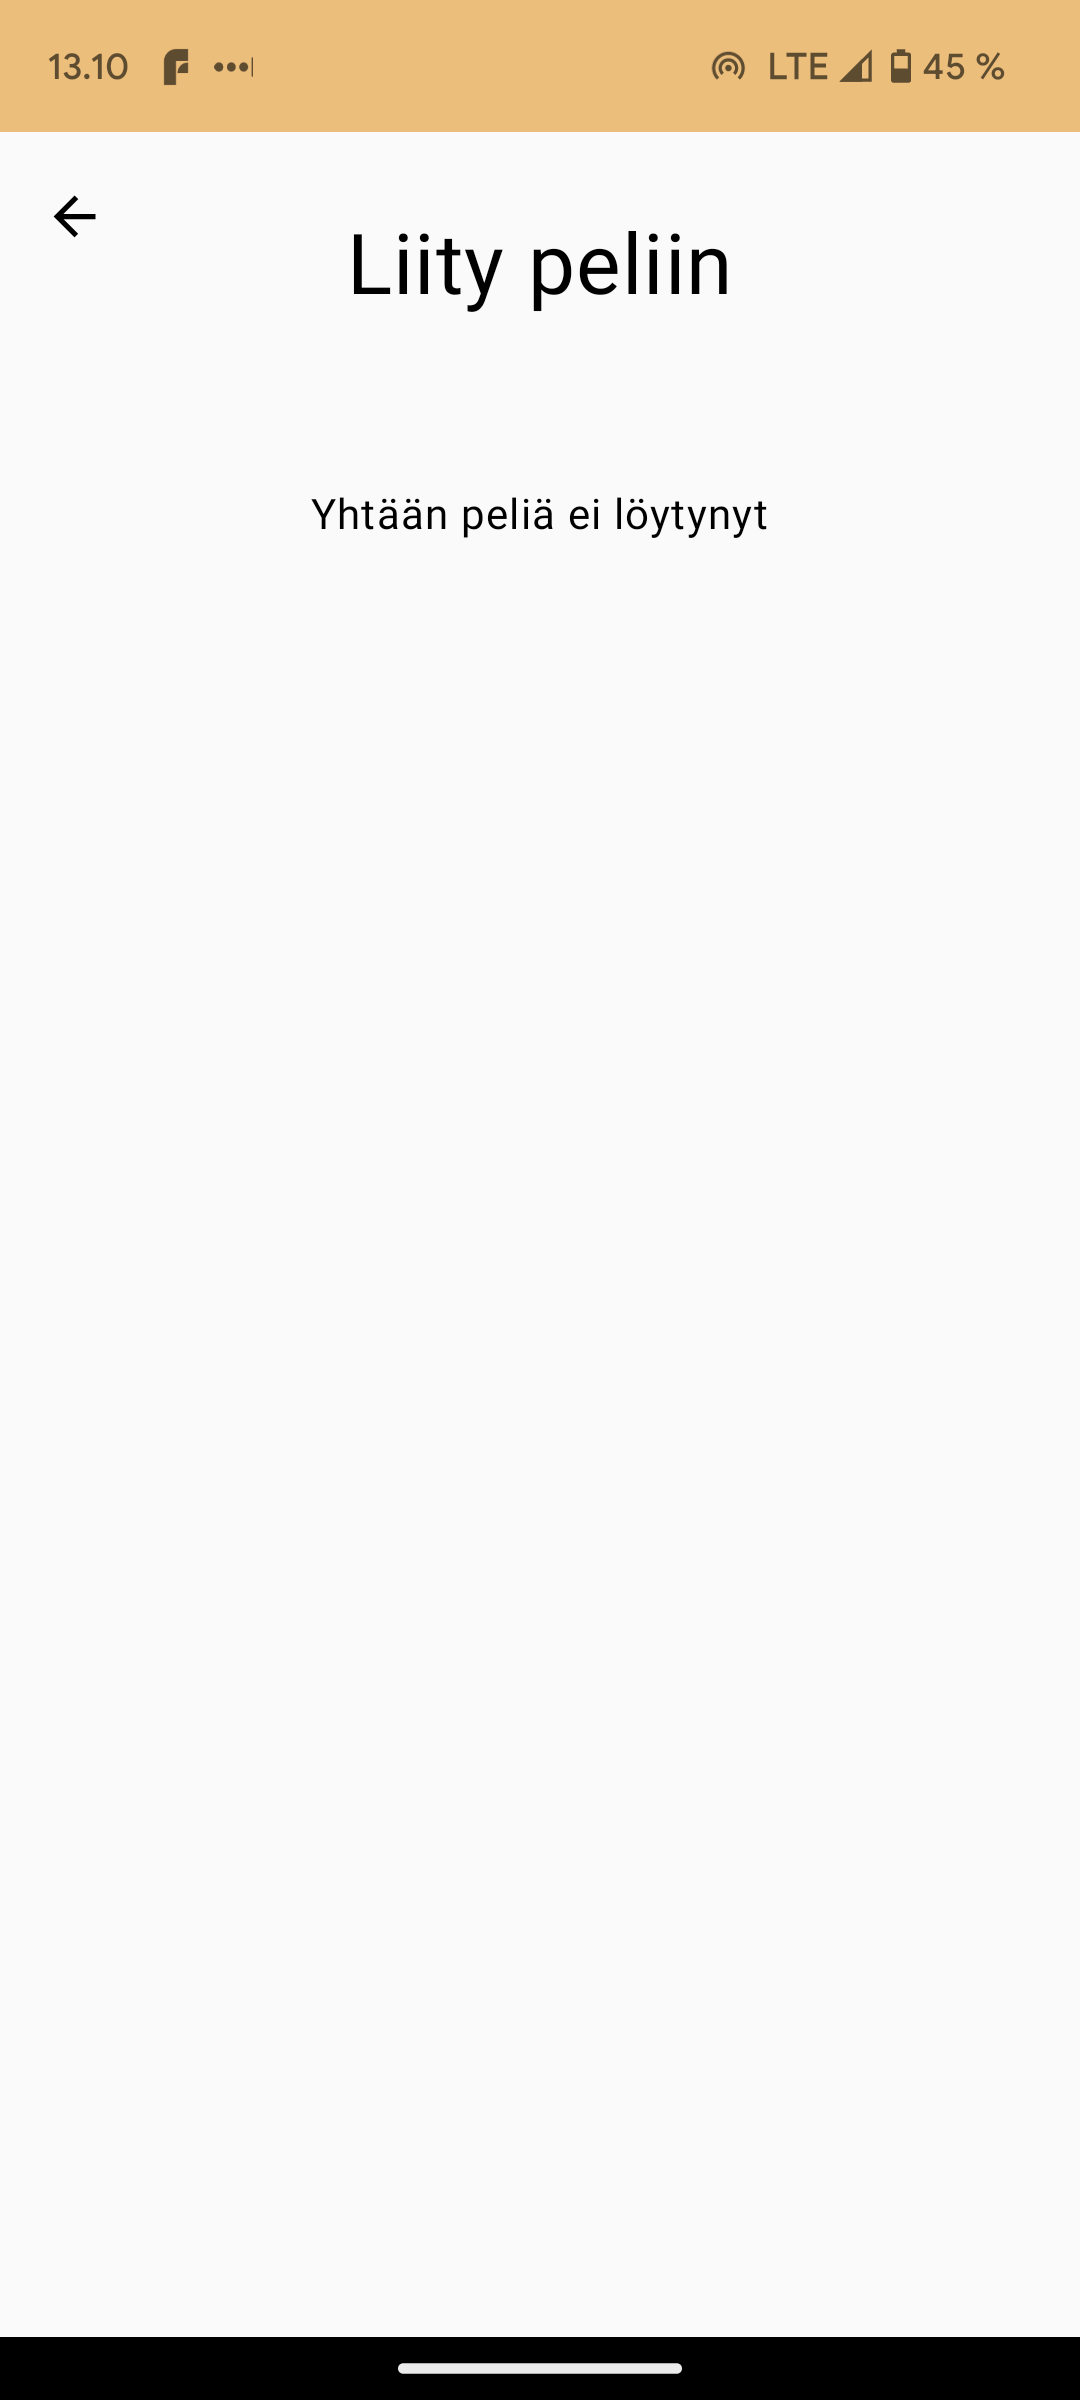
\includegraphics[width=\textwidth]{figures/screenshot-join-game.png}
            \caption{Keskeneräinen pelin liittymisnäkymä}
            \label{fig:screenshot-join-game}
      \end{minipage}
\end{figure}

Pelin luomisen jälkeen siirrytään pelinäkymään
(kuva \ref{fig:screenshot-add-players}), jossa saadaan lisättyä pelaajat peliin ja
sen jälkeen aloitettua pelaaminen. Pelaaja lisätään peliin antamalla pelaajan
nimi kuvan \ref{fig:screenshot-add-player} mukaisesti. Kun peli aloitetaan,
arvotaan pelaajille roolit ja näytetään ne kuvan
\ref{fig:screenshot-game-started} mukaisesti.

\begin{figure}[h!]
      \centering
      \begin{minipage}[t]{.3\textwidth}
            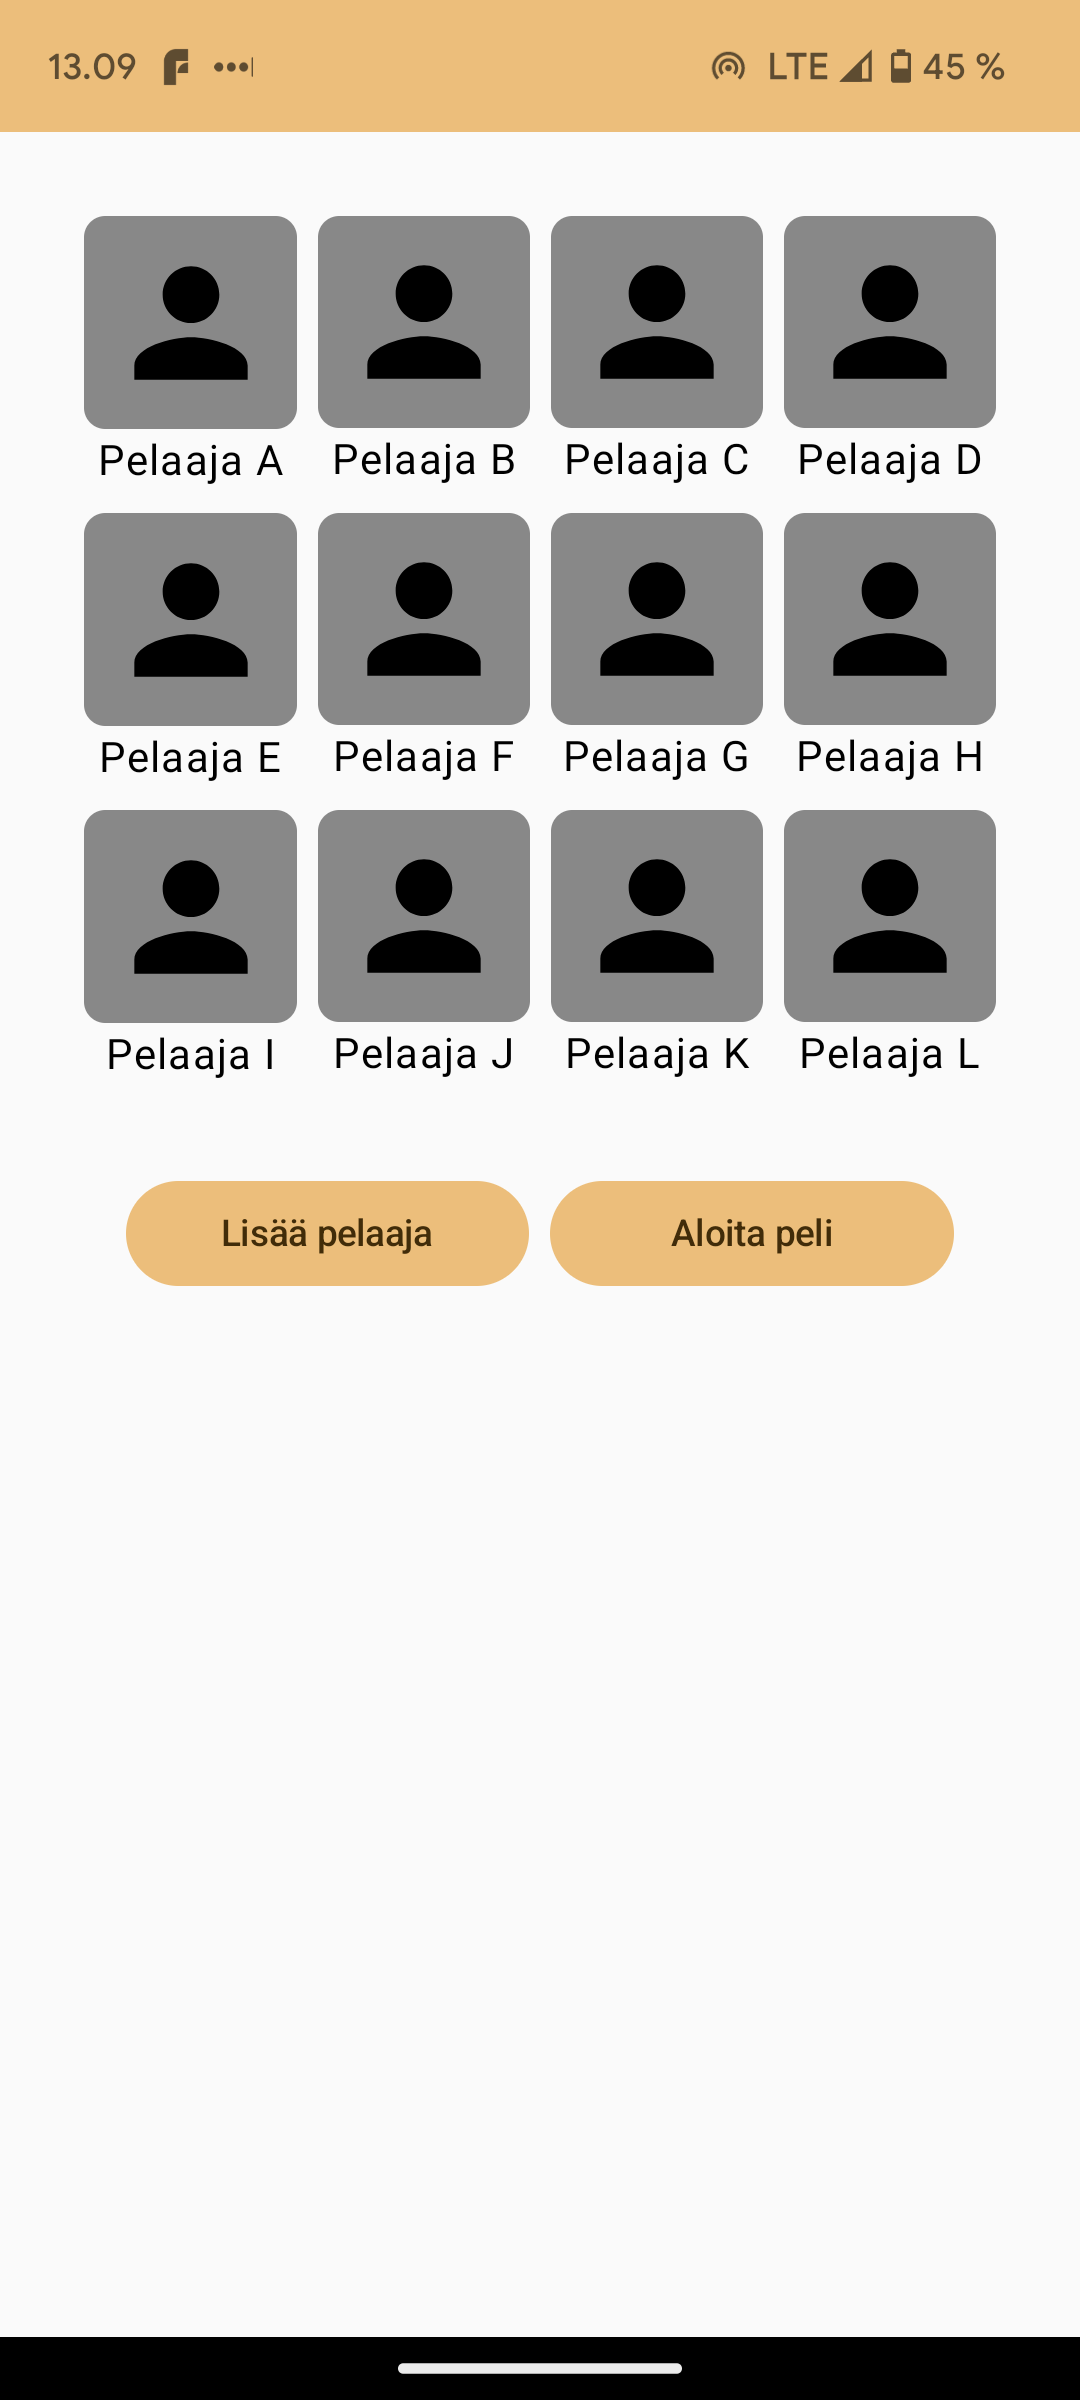
\includegraphics[width=\textwidth]{figures/screenshot-add-players.png}
            \caption{Pelaajien lisääminen ennen pelin aloittamista}
            \label{fig:screenshot-add-players}
      \end{minipage}
      \begin{minipage}[t]{.3\textwidth}
            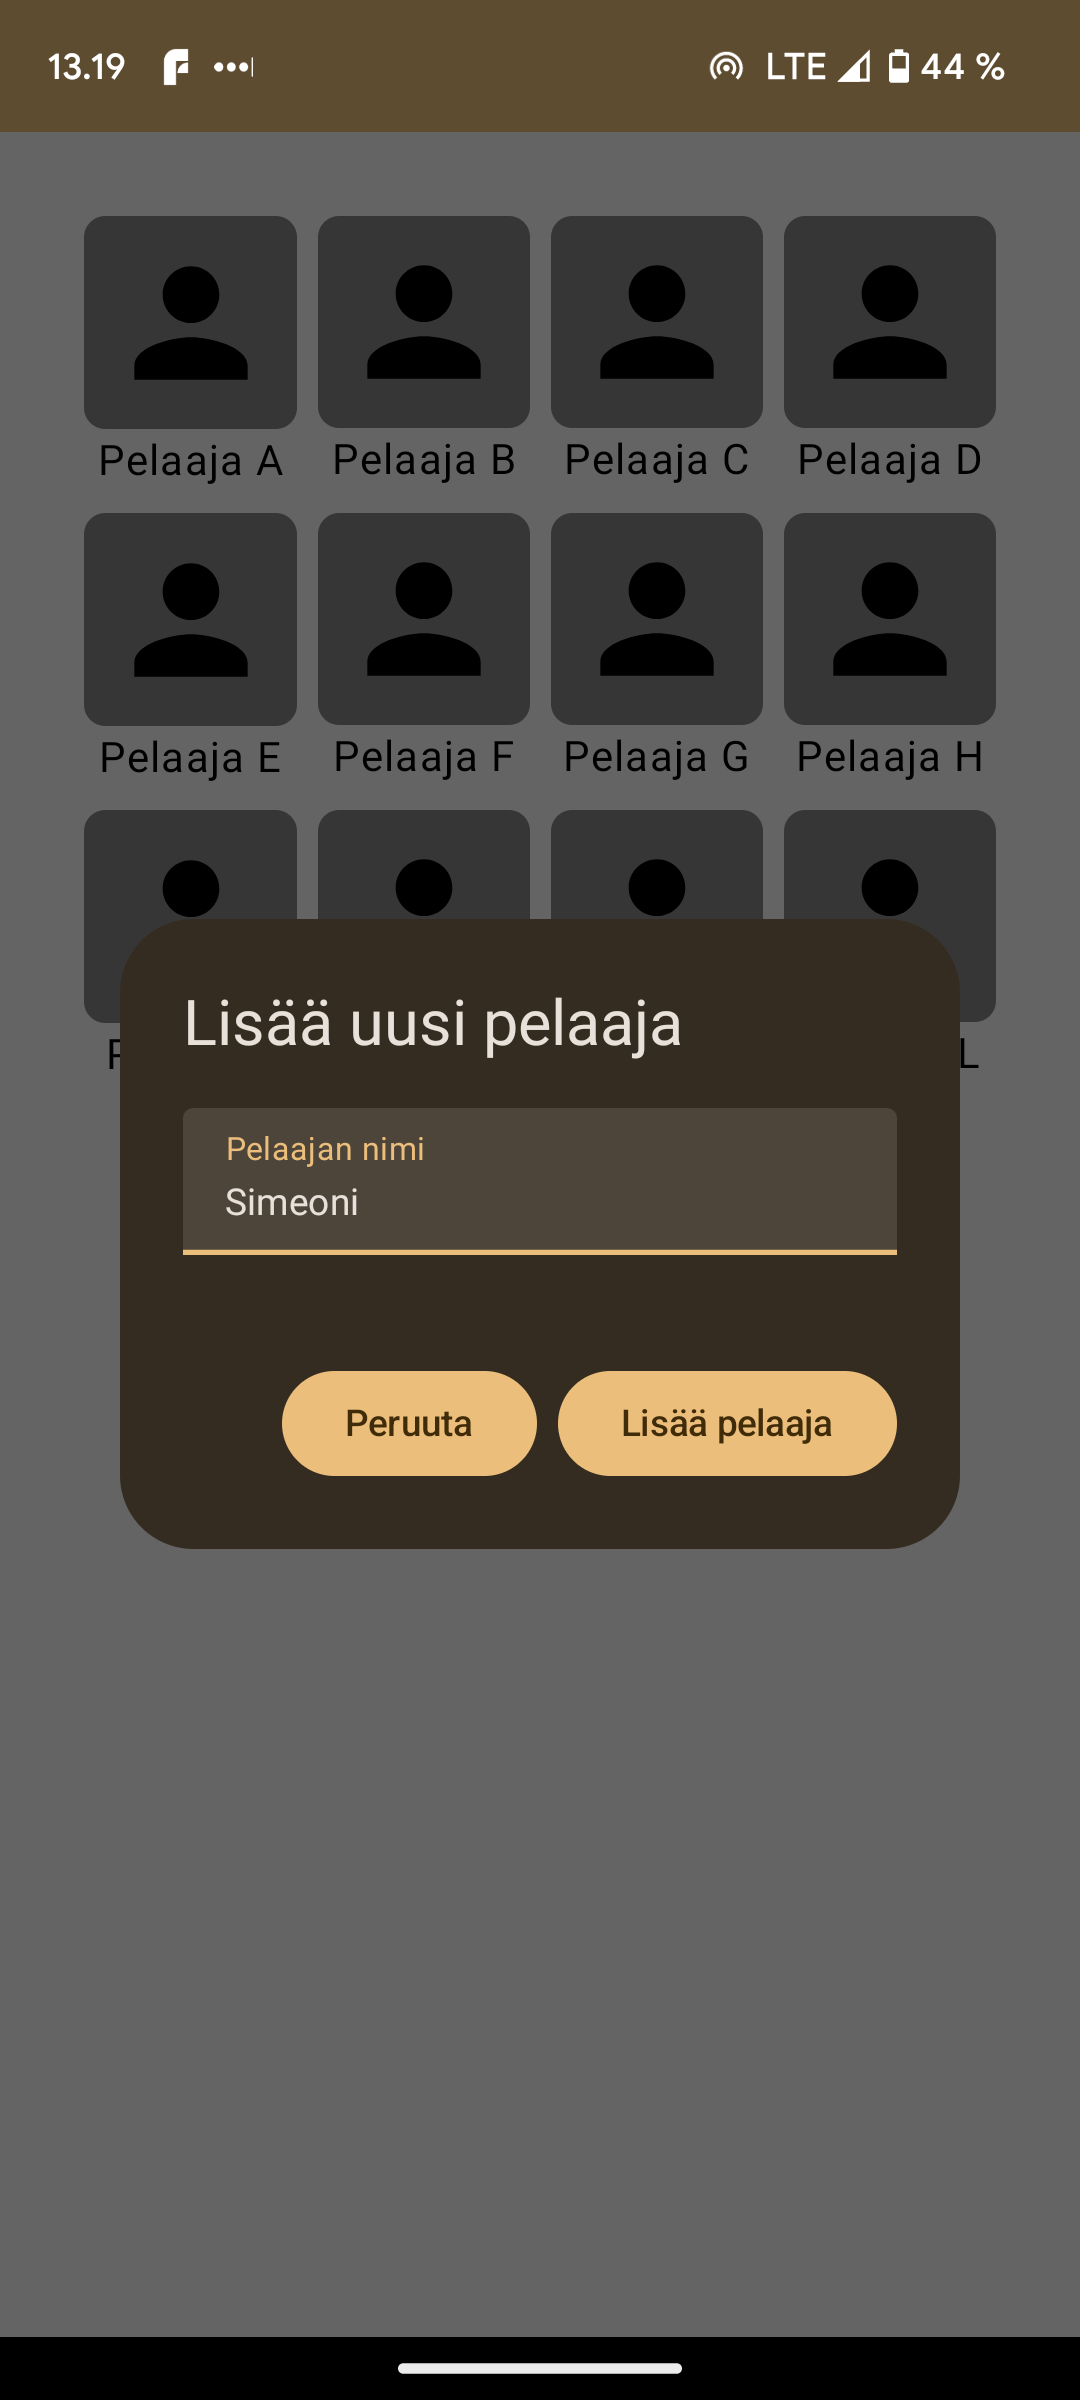
\includegraphics[width=\textwidth]{figures/screenshot-add-player.png}
            \caption{Pelaajan lisääminen}
            \label{fig:screenshot-add-player}
      \end{minipage}
      \begin{minipage}[t]{.3\textwidth}
            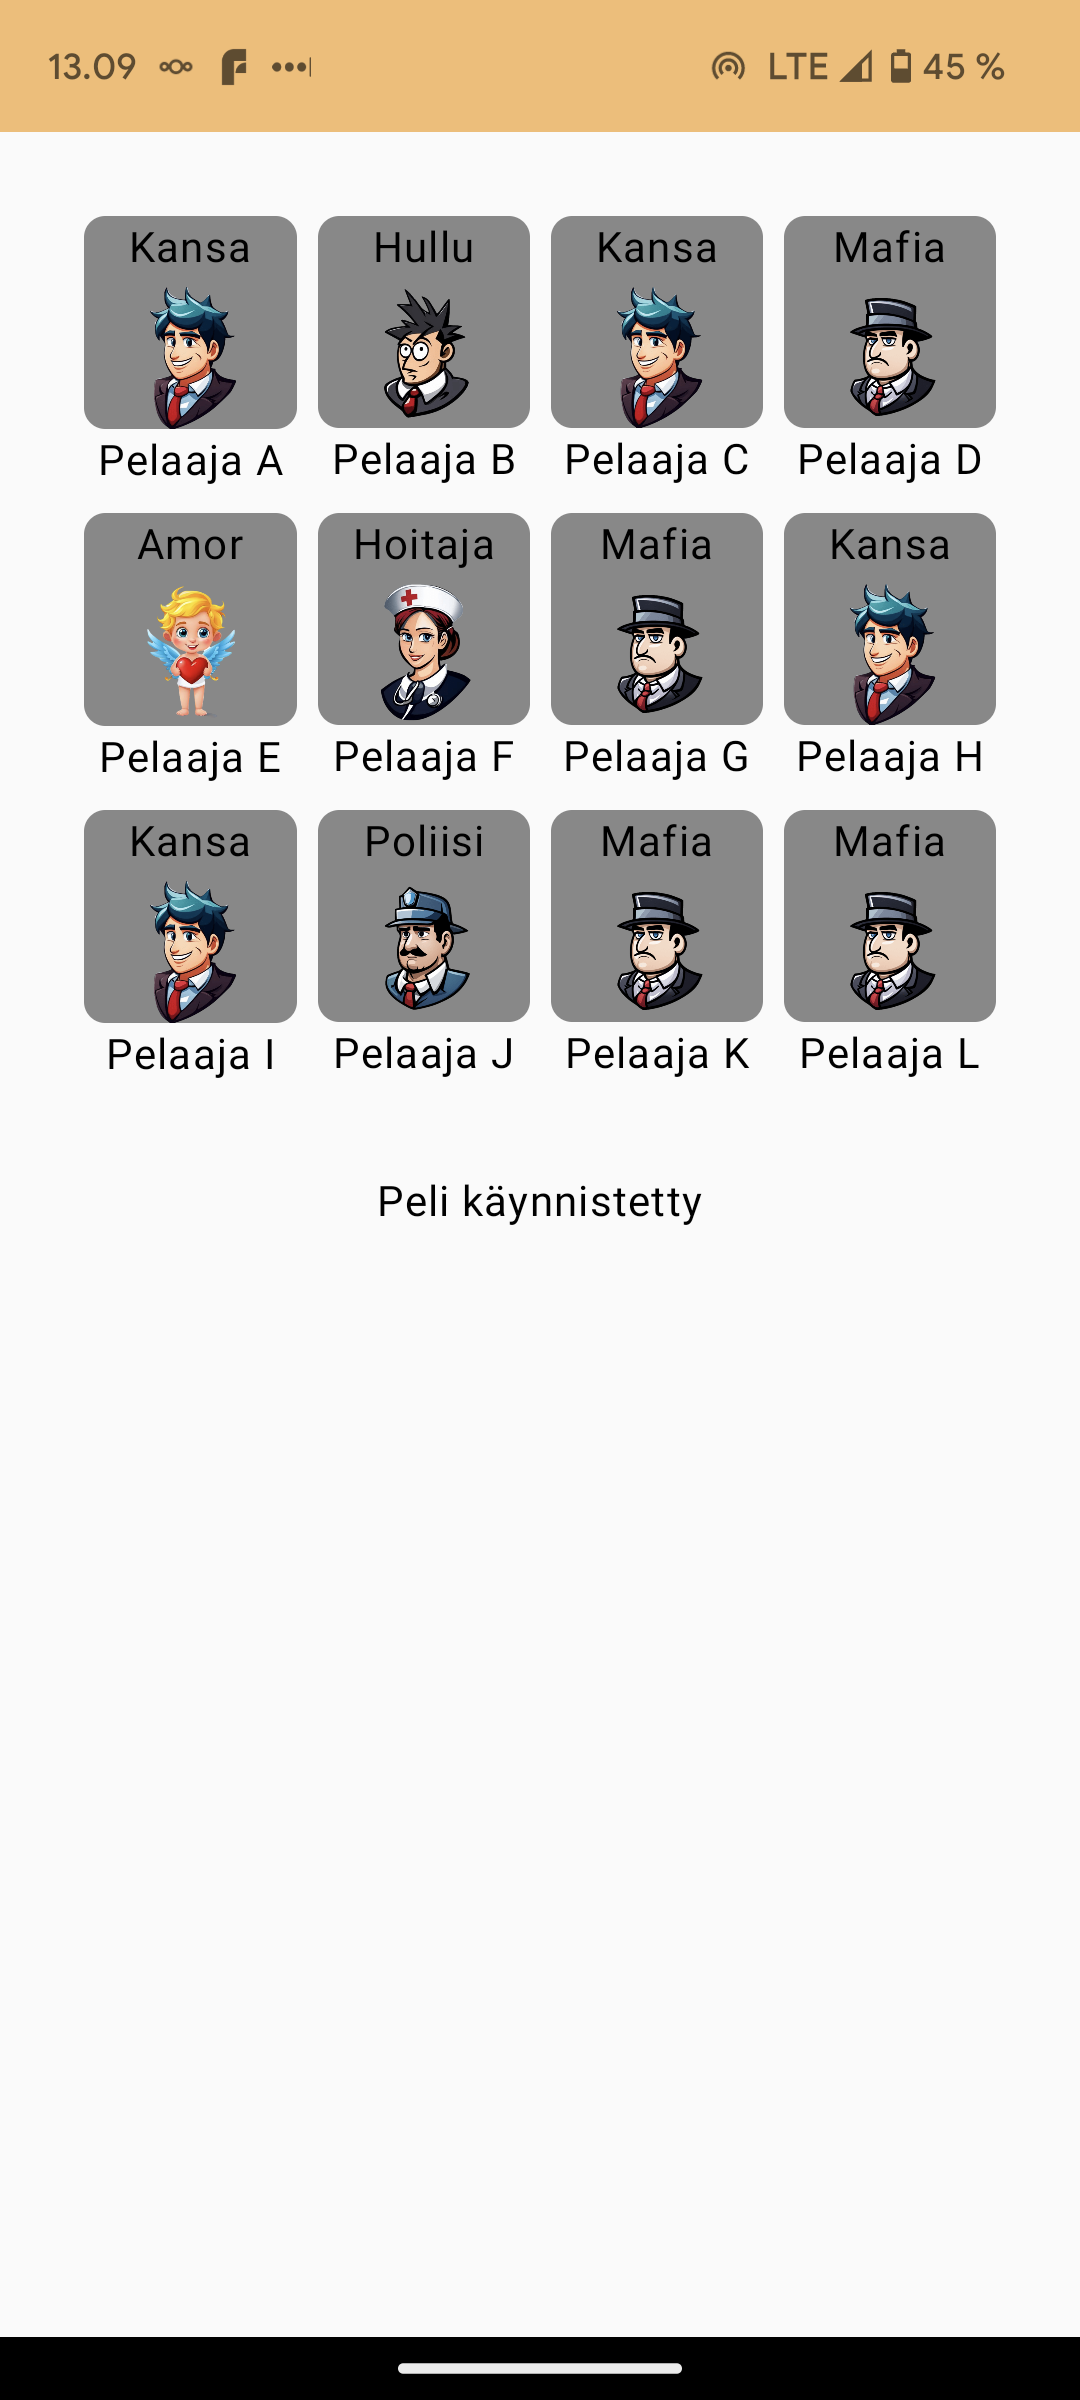
\includegraphics[width=\textwidth]{figures/screenshot-game-started.png}
            \caption{Näkymä pelin aloittamisen jälkeen}
            \label{fig:screenshot-game-started}
      \end{minipage}
\end{figure}

Pelaajien ja roolien tarkempia tietoja voi katsella painamalla kuvassa
\ref{fig:screenshot-game-started} näkyviä pelaajia, joka avaa kuvassa
\ref{fig:screenshot-card-details} näkyvät tiedot (näkyvät hiukan heikosti). Kun
pelaajia poistetaan pelistä, näkyvät pelaajat kuvan
\ref{fig:screenshot-game-running} mukaisesti. Lopulta kun peli on ohi, tulee
ilmoitus kuvassa \ref{fig:screenshot-game-over} näkyvällä tavalla.

\begin{figure}[h!]
      \centering
      \begin{minipage}[t]{.3\textwidth}
            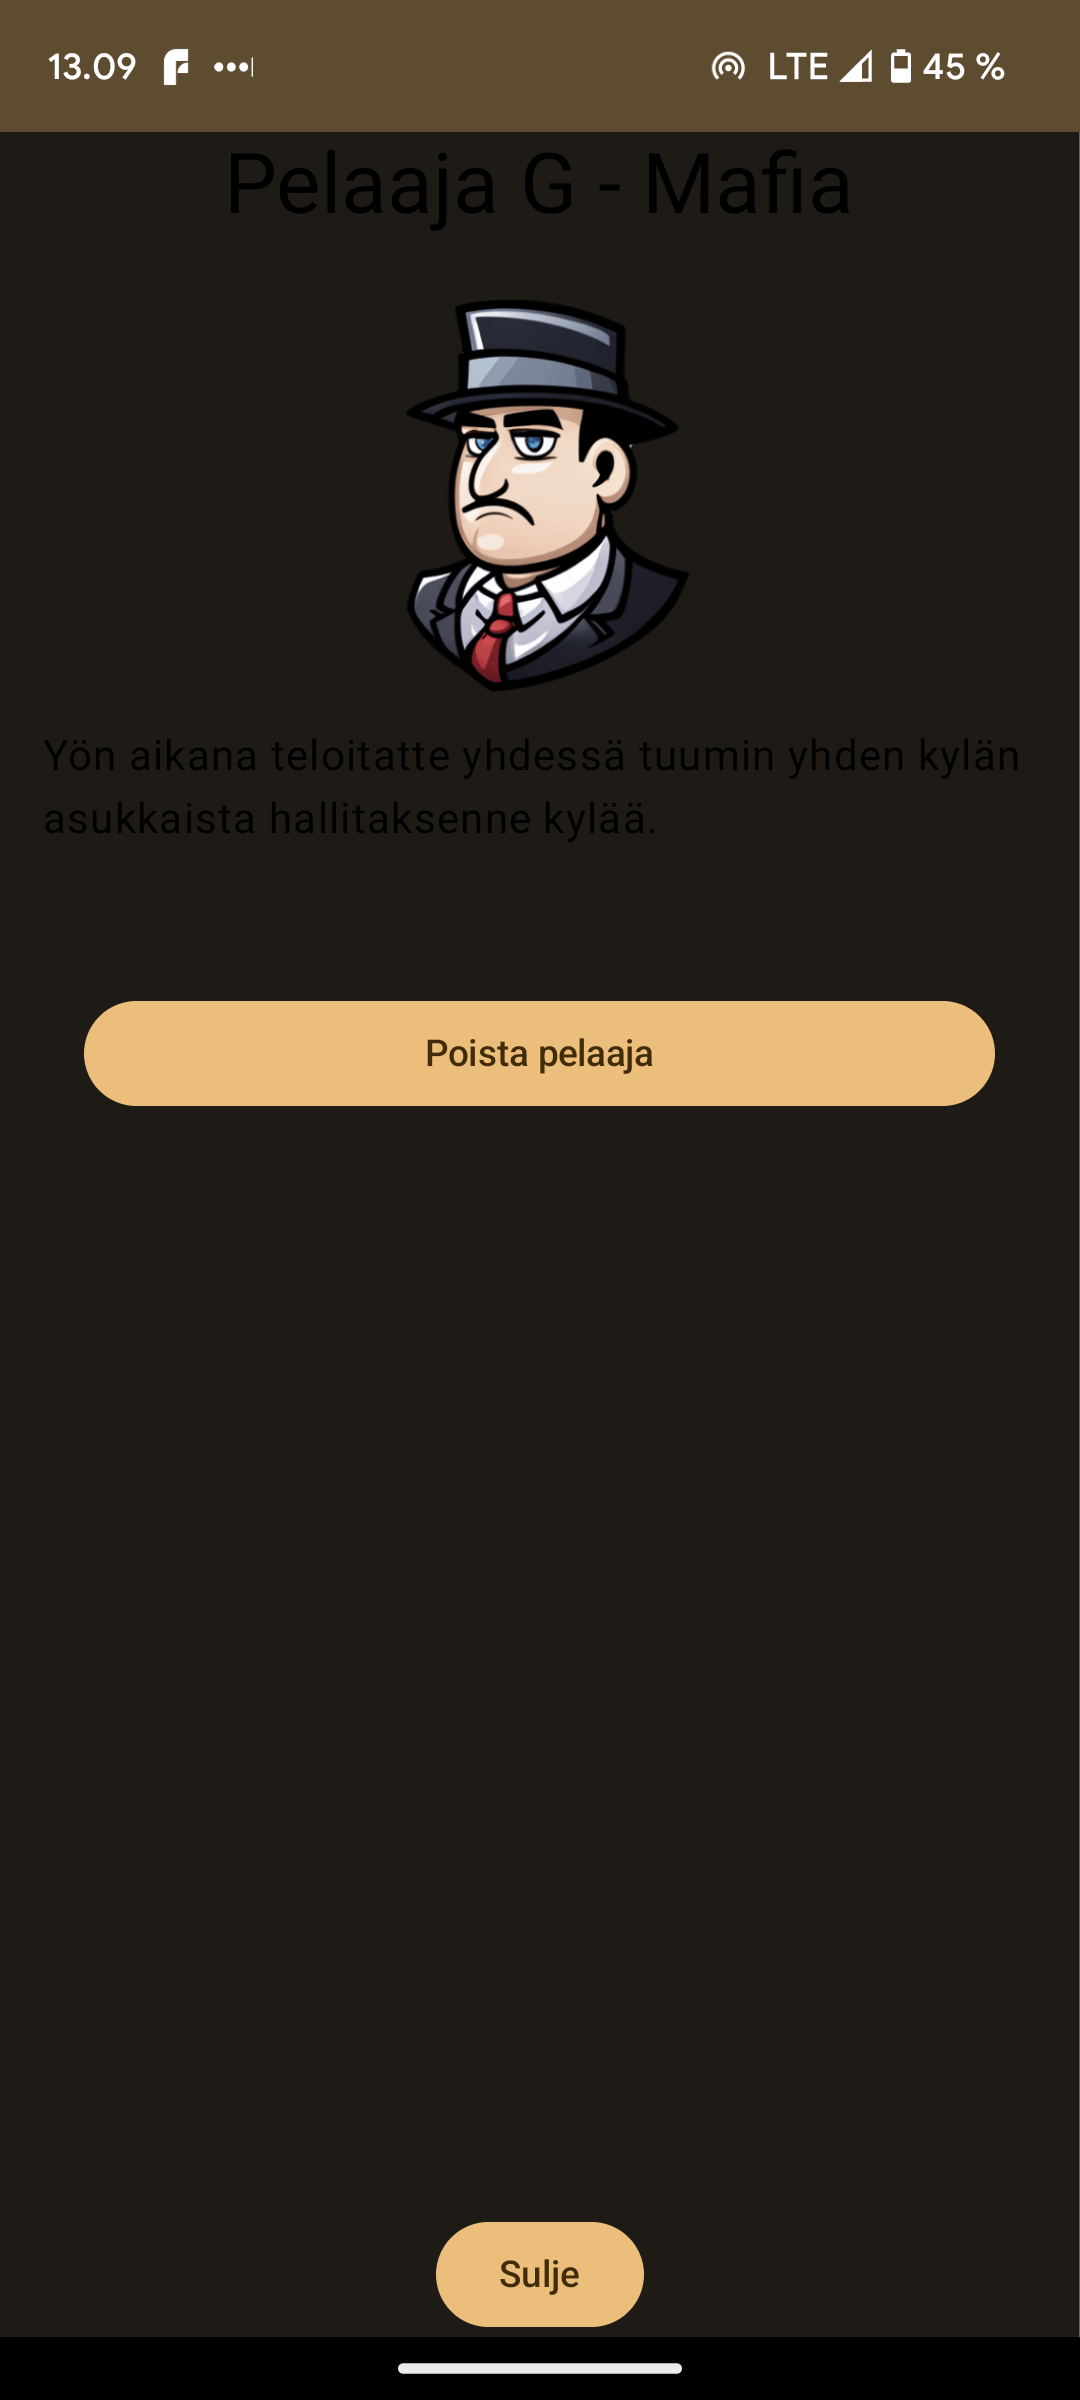
\includegraphics[width=\textwidth]{figures/screenshot-card-details.png}
            \caption{Pelaajien roolien esikatselu}
            \label{fig:screenshot-card-details}
      \end{minipage}
      \begin{minipage}[t]{.3\textwidth}
            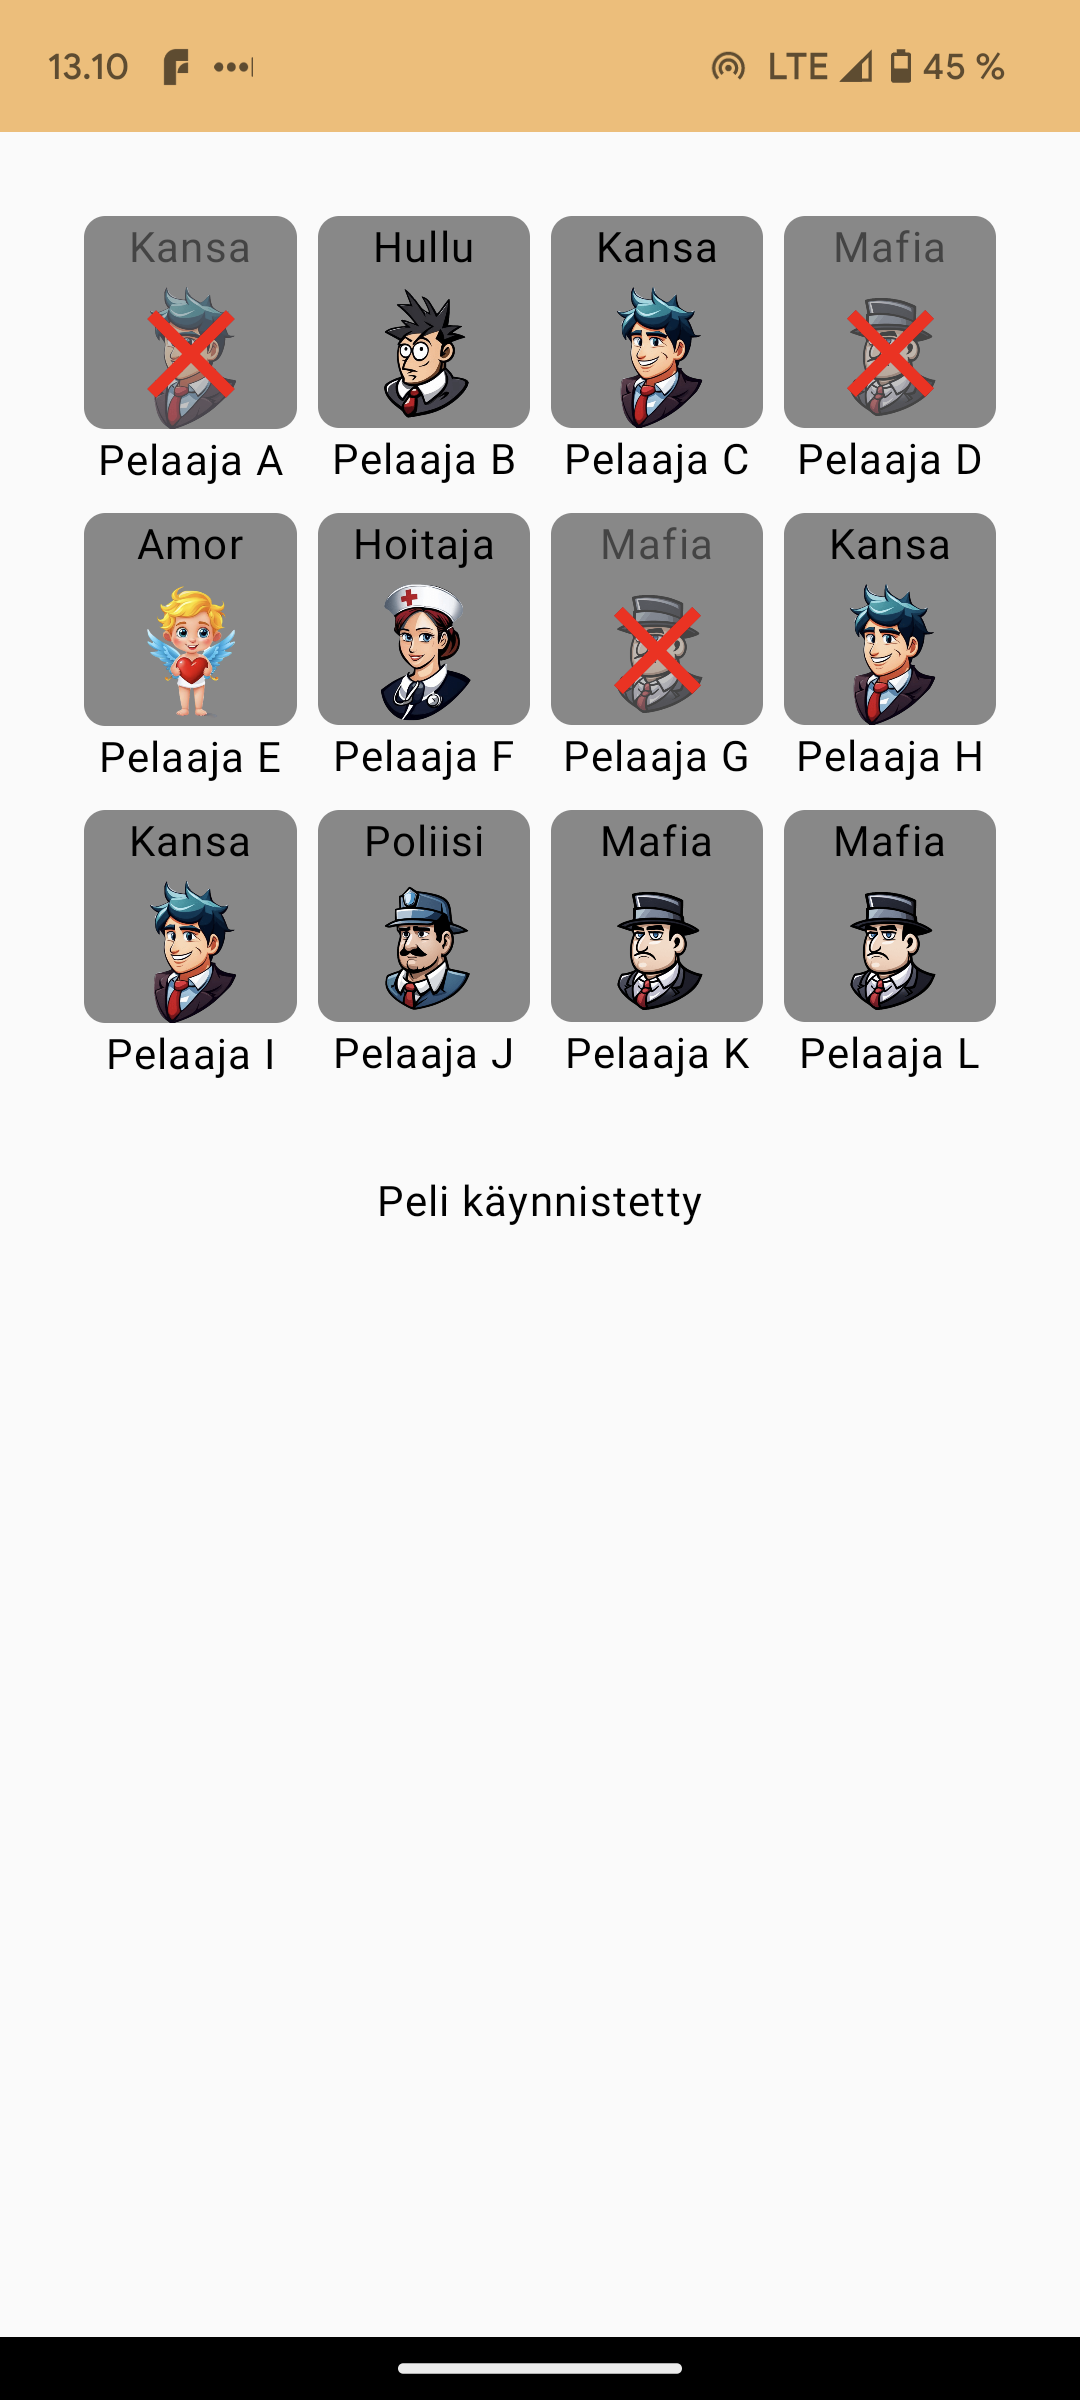
\includegraphics[width=\textwidth]{figures/screenshot-game-running.png}
            \caption{Esimerkki tilanteesta, jossa osa pelaajista poistettu pelistä}
            \label{fig:screenshot-game-running}
      \end{minipage}
      \begin{minipage}[t]{.3\textwidth}
            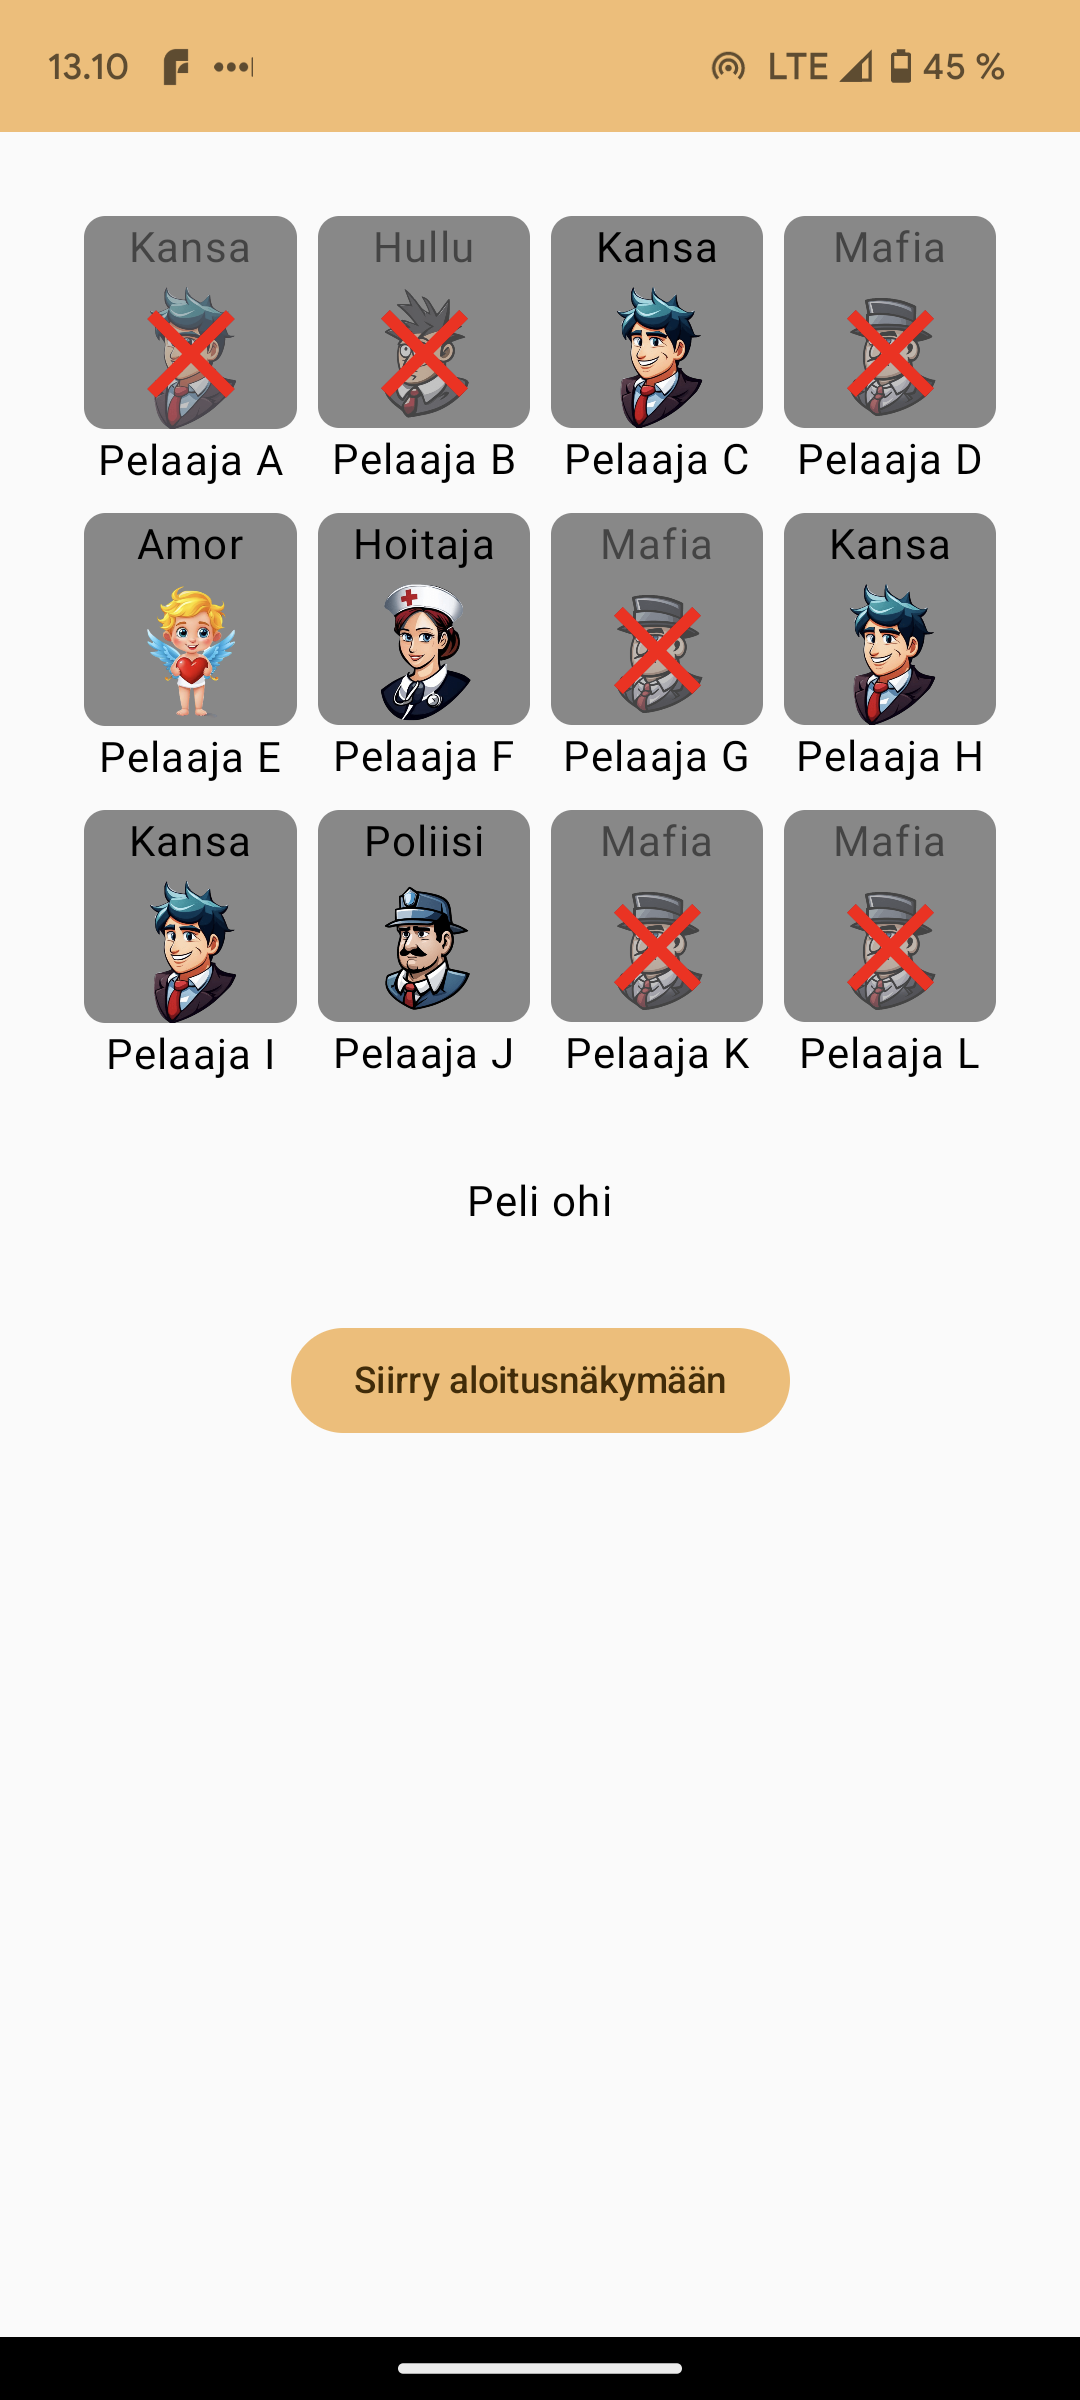
\includegraphics[width=\textwidth]{figures/screenshot-game-over.png}
            \caption{Esimerkki tilanteesta, jossa peli on päättynyt}
            \label{fig:screenshot-game-over}
      \end{minipage}
\end{figure}

\subsection{Projektin julkaisu}

Vaikka projektin on yhä selvästi keskeneräinen, julkaistaan sovellus sisäiseen
testaukseen sellaisenaan, jotta päästään perehtymään sovellusten
julkaisemiseen. Androidilla Play-kaupan ollessa ilmeisesti ylivoimaisesti
käytetyin, perehdytään sinne julkaisuun, ilman että sen tarkemmin perehdytään
esimerkiksi Huawein sovelluskauppaan.

Sovelluksen julkaiseminen Play kauppaan vaatii kehittäjätilin Play consoleen.
Kehittäjätilin luonti vaatii tietojen antamisen, henkilöllisyyden maksamisen
ja pienehkö maksun. Lisäksi tilin luonnissa kysytään joitakin tietoja, joilla
pyritään ilmeisesti estämään mm. väärinkäytöksiä. Näitä ovat esimerkiksi
kehittäjätilin käyttötarkoitus (henkilökohtainen vs. yritys) ja kuinka paljon
on tarkoitus julkaista sovelluksia.

Consolesta löytyy huomattavasti asioita, joihin lienee hyvä perehtyä
ajankanssa, mutta onneksi julkaisun luomisen yhteydessä tulee esille kattava 13
kohdan lista kaikista asioita, jotka tulee tehdä ennen kuin sovellus voidaan
julkaista edes sisäiseen testaukseen. Näistä ehkä eniten työtä tuottaa
tietosuojakäytäntö, jonka ei pitäisi ilmeisesti olla pakollinen, mutta data
turvallisuus kysely vaatii sen kuitenkin pakollisena. Nopeasti toki saadaan
tehtyä Github Pagesiin pyörimään kevyet sivut, joilta löytyy
tietosuojakäytäntö. Toki jotta samalla tulee kokeiltua jotain uutta, jonka
pitäisi toimia hyvin juurikin näin kevyisiin staattisiin sivuihin, valitaan
käytettäväksi Jekyll, jota Github suosittelee projektille dokumentaatiosivuiksi
yms. Jotta asiat eivät olisi tarpeeksi helppoja niin Jekyliin asentamisen
yhteydessä selviää, että olen confannut rubyn gemien asentamisen väärin ja
tästä aiheutuu virhe Jekylin kanssa. Tähän toki löytyy onneksi nopeasti
ratkaisu \parencite{StakOverflowRubyGemsPermissionsDenied} ja päästää
asentamaan Jekyll. Toki Jekylillä sivustoa staattista luodessa saadaan virhe,
ettei kirjastot ole yhteensopivia vaan vaativat uudemman rubyn version, jota
ei ole suoraan saatavilla Debian 11:lla tarjolla olevista repositoryista. Jotta
julkaisu saadaan etenemään niin tässä kohtaa on hyvä vaihtaa käyttämään jotain
ennestään tuttua ja toimivaa eli itselleni NextJs:ää. NextJs:ssä nopeahkosti
staattiset sivut, joissa etusivu on kuva tekstillä "Sivut ovat yhä työnalla!"
ja alasivuksi tietosuojakäytäntö, joka voidaan linkata Play Consoleen. Sivusto
saadaan pystyy Github Pagesiin käyttämällä valmista pohjaa Github Actioneihin ja
muokkaamalla se tähän tilanteeseen sopivaksi. Sivuston sekä Github Actioneiden
koodi on mukana git repossa projektin alla. Sivusto löytyy osoitteesta:
https://mafioso.app/ ja tietosuojakäytäntö https://mafioso.app/tietosuoja.

Tunnetusti yhden asian korjaamisen yhteydessä ilmenee toinen ongelma, jonka
korjauksen yhteydessä kolmas asia jne. Tällä kertaa tietosuojakäytännön
luominen osoittautui juuri tällaiseksi, sillä mafioso.app-verkkotunnuksen DNS-
tietueet olivat yhä vanhalla DNS palvelimillani, joten siirtäminen oli hiukan
isompi operaatio ja aikaa vievä, mutta odotellessa DNS välimuistien
tyhjentymistä, sai siistittyä uuden sivuston etusivua ja tehtyä siitä samalla
paremmin responsiivisen.

Kehittäjätilin vahvistaminen luvattiin toteuttaa kahdessa arkipäivässä, joten
kaiken muun jälkeen jäi julkaiseminen odottamaan tuota vahvistusta. Vahvistus
tuli tosiaan kahden arkipäivän sisällä ja tämän jälkeen sovellus oli
mahdollista julkaista sisäiseen testaukseen. Sisäisessä testauksessa
sovelluksen pystyy jo samantien asentamaan Play-kaupan kautta, mutta sovellus
näkyy yhä automaattisesti generoidulla nimellä ja kuvakkeella, kunnes sovellus
on saatu vahvistettua. Tämä toki riitti siihen, että sovelluksen sai asennettua
myös Play-kaupan kautta eikä tarvinnut asentaa Android Studion avulla. Sovellus
on yhä tätä kirjoittaessa (ja todennäköisesti palauttaessa) tarkistuksessa,
sillä siihen arvioitu aika on viikko.

\subsection{Tuntikirjanpito}

Oheiseen taulukkoon \ref{tab:project-working-hours} on koottu projektin
tekemiseen käytetyt tunnit vastaavasti kuin aiemmissakin tuntikirjanpidoissa.

\begin{table}[H]
    \centering
    \label{tab:project-working-hours}
    \begin{tabular*}{\linewidth}{@{\extracolsep{\fill}} l c c c r }
        \textbf{Päivämäärä} & \textbf{Aloitettu} & \textbf{Lopetettu} & \textbf{Määrä} \\
        \hline
        25.07.2023 & 06:40 & 11:40 & 5h 00m \\
        25.07.2023 & 12:00 & 12:20 &    20m \\
        25.07.2023 & 15:15 & 17:30 & 2h 15m \\
        26.07.2023 & 08:20 & 10:30 & 2h 10m \\
        26.07.2023 & 10:50 & 11:30 &    40m \\
        26.07.2023 & 13:00 & 21:10 & 7h 10m \\
        27.07.2023 & 10:25 & 10:35 &    10m \\
        \hline
        \multicolumn{3}{l}{\textbf{Yhteensä}} & \textbf{XXh XXm} \\
    \end{tabular*}
\end{table}
